\newpage
\section{Конструкторский раздел}
В этом разделе будут подробно описаны основные функции библиотеки, приведены схемы их работы.

	\subsection{Общий алгоритм}
	Общий алгоритм выглядит следующим образом (рисунок \ref{fig1:image}):
	
	\begin{figure}[ph!]
		\centering
		\begin{center}
			{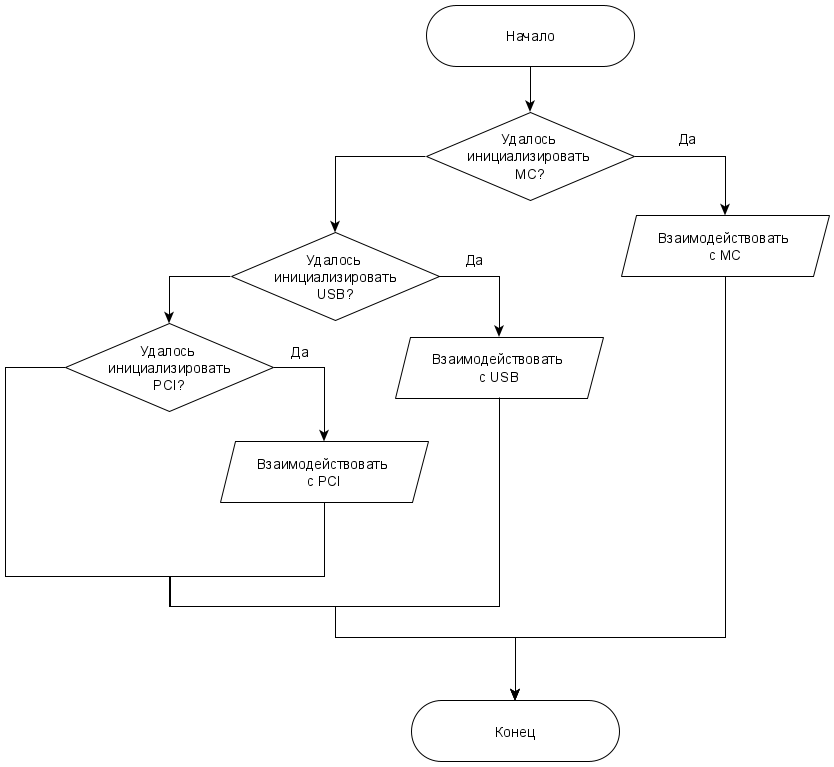
\includegraphics[scale=0.5]{schemes/general.png}}
			\caption{Общий алгоритм}
			\label{fig1:image}
		\end{center}
	\end{figure}


	\subsection{USB}
	\subsubsection{Функция инициализации (USB$\_$Open)}
	
	Схема изображена на рисунке \ref{fig2:image}.
	
	\begin{figure}[ph!]
		\centering
		\begin{center}
			{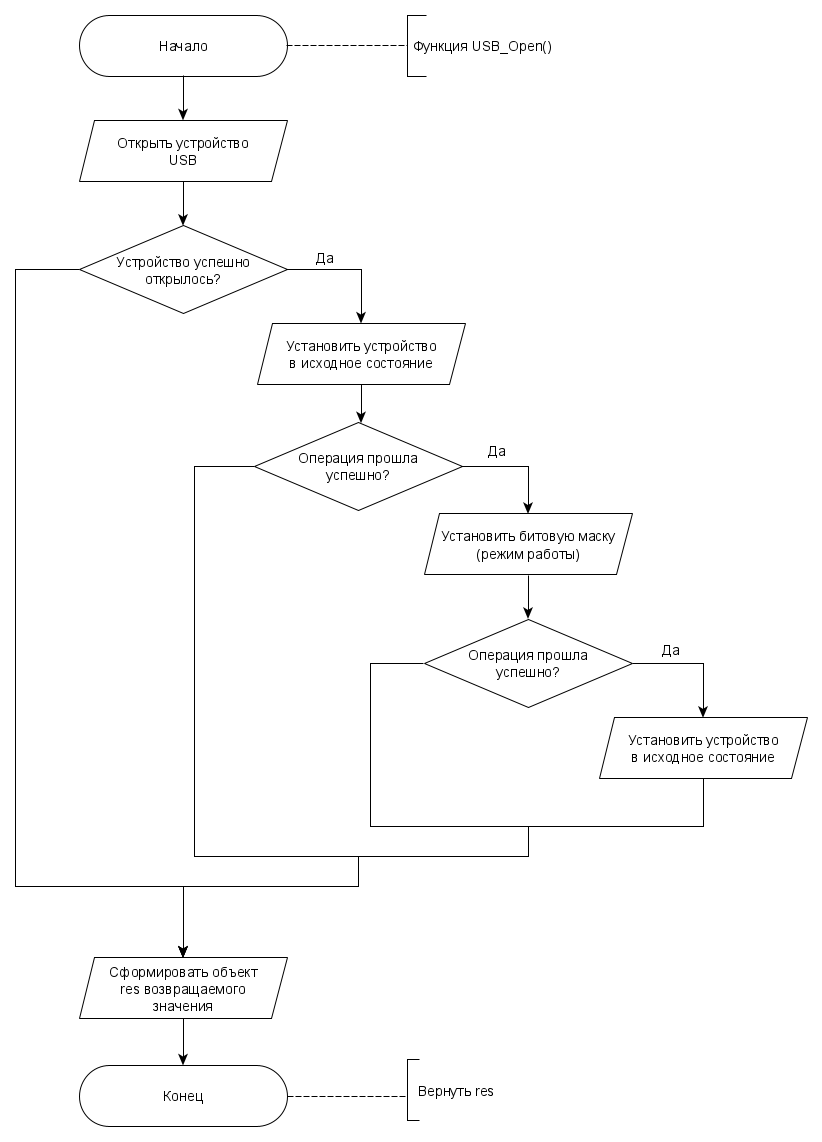
\includegraphics[scale=0.5]{schemes/usb_open.png}}
			\caption{USB$\_$Open()}
			\label{fig2:image}
		\end{center}
	\end{figure}

	\subsubsection{Прекращение работы с USB (USB$\_$Close)}
	
	Схема изображена на рисунке \ref{fig3:image}.
	
	\begin{figure}[ph!]
		\centering
		\begin{center}
			{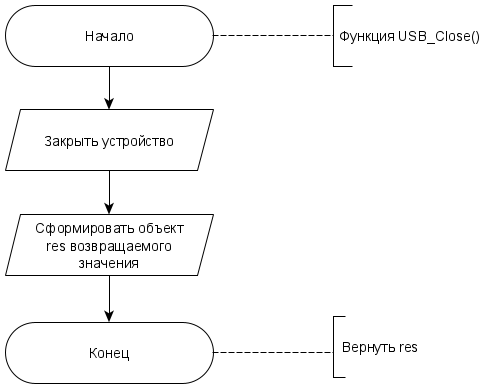
\includegraphics[scale=0.5]{schemes/usb_close.png}}
			\caption{USB$\_$Close()}
			\label{fig3:image}
		\end{center}
	\end{figure}

	\subsubsection{Функция записи данных в устройство USB-КМБО (USB$\_$Write)}

	Схема изображена на рисунке \ref{fig4:image}.
	
	\begin{figure}[ph!]
		\centering
		\begin{center}
			{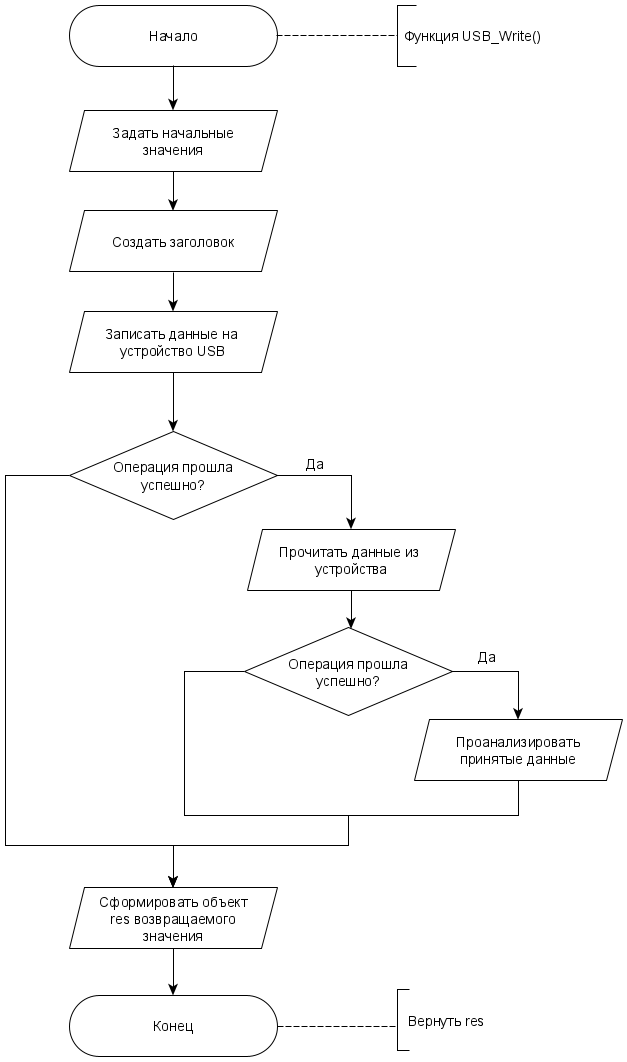
\includegraphics[scale=0.5]{schemes/usb_write.png}}
			\caption{USB$\_$Write()}
			\label{fig4:image}
		\end{center}
	\end{figure}

	\newpage

	\subsubsection{Функция чтения данных из устройства USB-КМБО (USB$\_$Read)}
	
	Схема изображена на рисунке \ref{fig5:image}.
	
	\begin{figure}[ph!]
		\centering
		\begin{center}
			{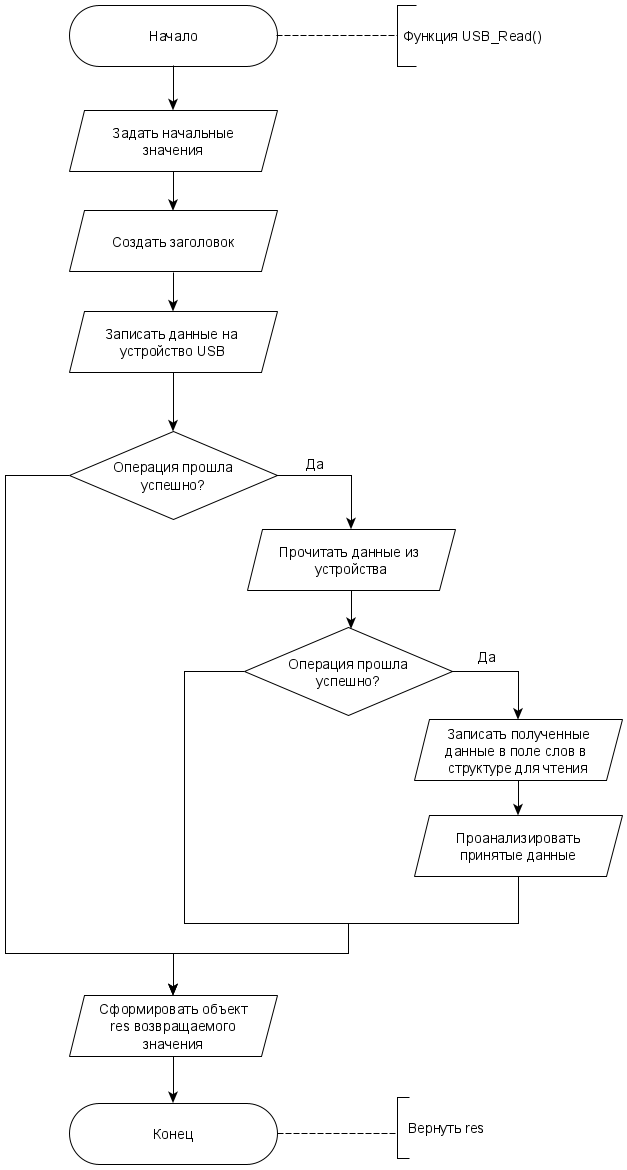
\includegraphics[scale=0.5]{schemes/usb_read.png}}
			\caption{USB$\_$Read()}
			\label{fig5:image}
		\end{center}
	\end{figure}

	\subsection{PCI}
	\subsubsection{Функция инициализации (PCI$\_$Open)}
	
	Схема изображена на рисунке \ref{fig6:image}.
	
	\begin{figure}[ph!]
		\centering
		\begin{center}
			{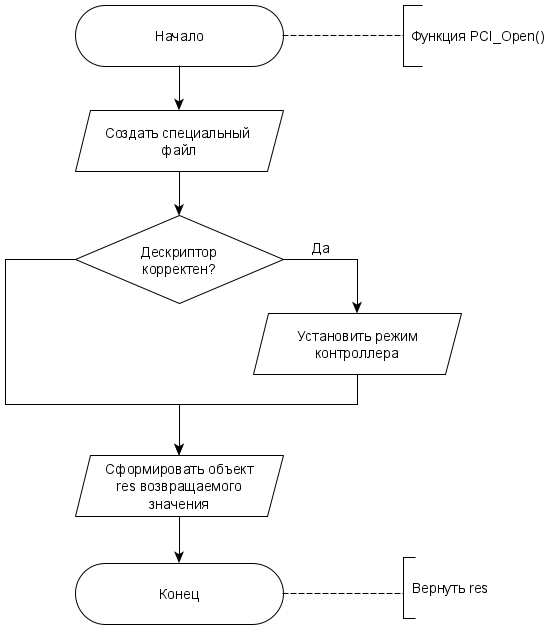
\includegraphics[scale=0.5]{schemes/pci_open.png}}
			\caption{PCI$\_$Open()}
			\label{fig6:image}
		\end{center}
	\end{figure}

	\newpage

	\subsubsection{Прекращение работы с PCI (PCI$\_$Close)}

	Схема изображена на рисунке \ref{fig7:image}.
	
	\begin{figure}[ph!]
		\centering
		\begin{center}
			{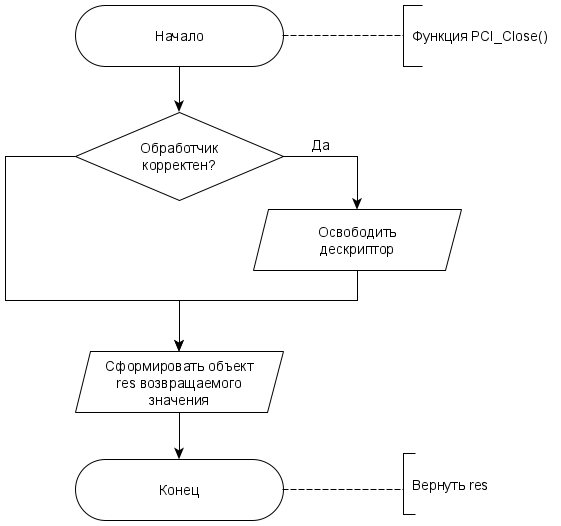
\includegraphics[scale=0.5]{schemes/pci_close.png}}
			\caption{PCI$\_$Close()}
			\label{fig7:image}
		\end{center}
	\end{figure}

	\newpage
	\subsubsection{Функция записи данных в устройство PCI-КМБО (PCI$\_$Write)}

	Схема изображена на рисунке \ref{fig8:image}.
	
	\begin{figure}[ph!]
		\centering
		\begin{center}
			{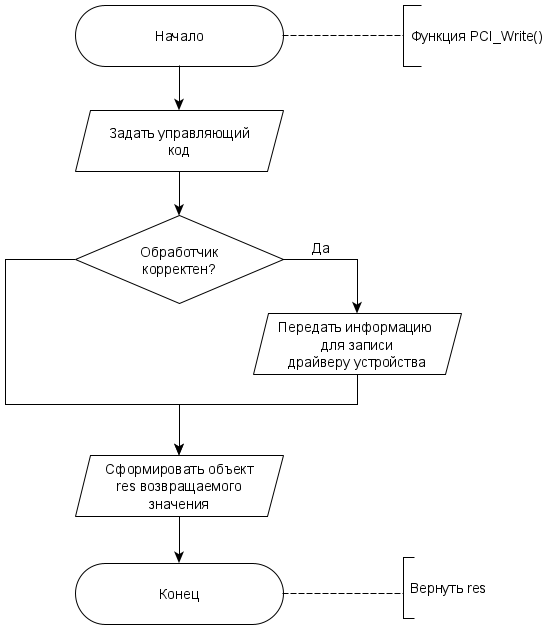
\includegraphics[scale=0.5]{schemes/pci_write.png}}
			\caption{PCI$\_$Write()}
			\label{fig8:image}
		\end{center}
	\end{figure}

	\newpage
	
	\subsubsection{Функция чтения данных из устройства PCI-КМБО (PCI$\_$Read)}
	
	Схема изображена на рисунке \ref{fig9:image}.
	
	\begin{figure}[ph!]
		\centering
		\begin{center}
			{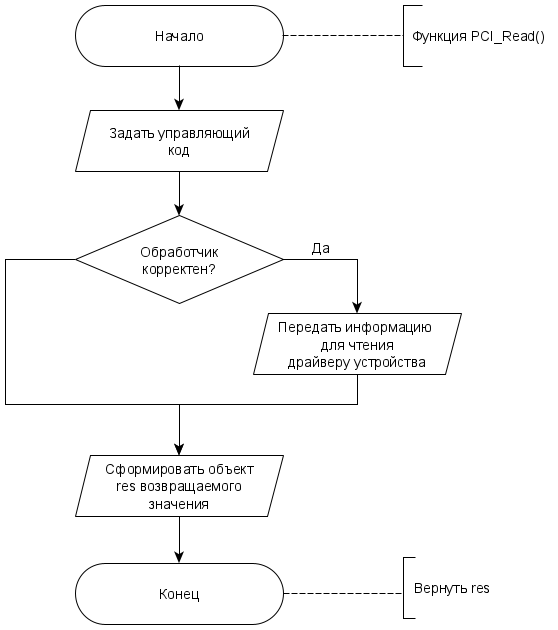
\includegraphics[scale=0.5]{schemes/pci_read.png}}
			\caption{PCI$\_$Read()}
			\label{fig9:image}
		\end{center}
	\end{figure}

	\subsection{Ethernet-КМБО}
	\subsubsection{Функция инициализации (MC$\_$Open)}
	
	Схема изображена на рисунке \ref{fig10:image}.
	
	\begin{figure}[ph!]
		\centering
		\begin{center}
			{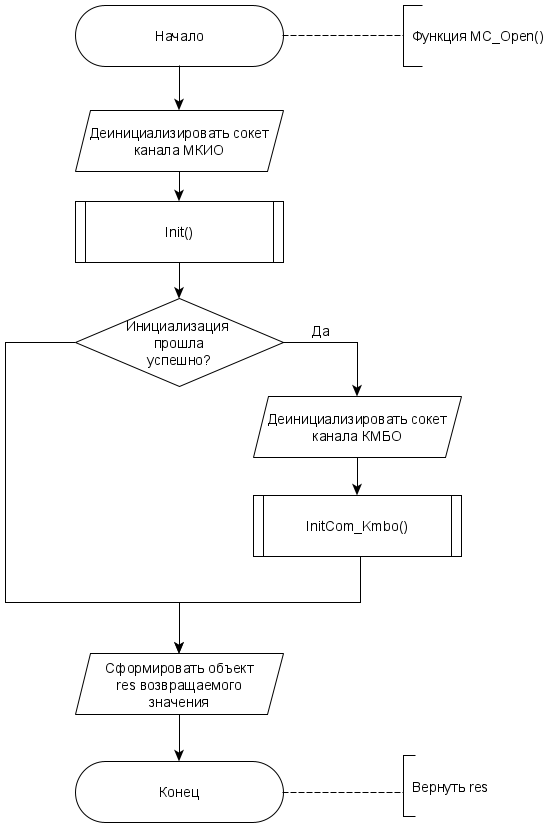
\includegraphics[scale=0.5]{schemes/mc_open.png}}
			\caption{MC$\_$Open()}
			\label{fig10:image}
		\end{center}
	\end{figure}

	\newpage

	\subsubsection{Прекращение работы с MC (MC$\_$Close)}
	
	Схема изображена на рисунке \ref{fig11:image}.
	
	\begin{figure}[ph!]
		\centering
		\begin{center}
			{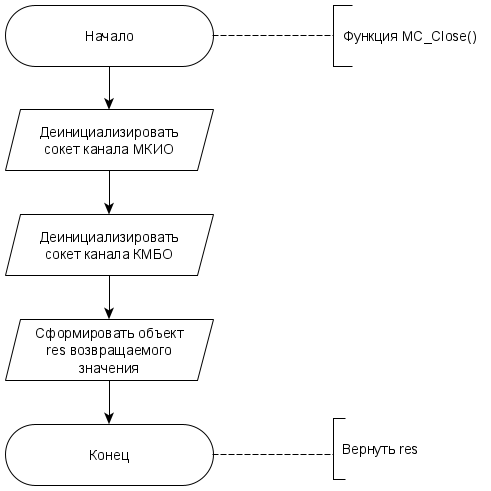
\includegraphics[scale=0.5]{schemes/mc_close.png}}
			\caption{MC$\_$Close()}
			\label{fig11:image}
		\end{center}
	\end{figure}

	\newpage
	\subsubsection{Функция записи данных в устройство MC-КМБО (MC$\_$Write)}
	
	Схема изображена на рисунке \ref{fig12:image}.
	
	\begin{figure}[ph!]
		\centering
		\begin{center}
			{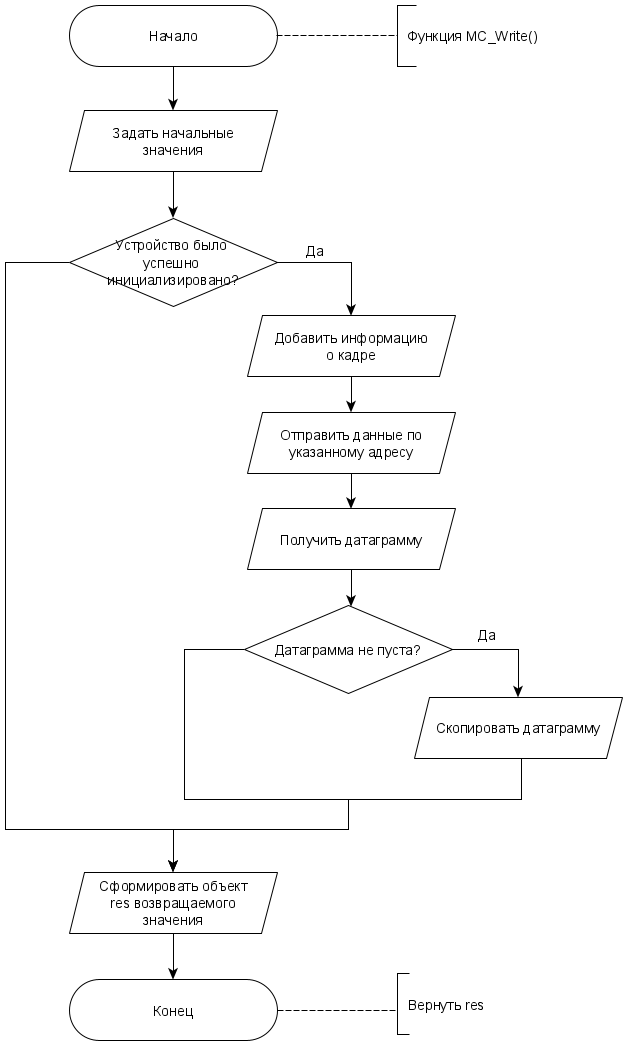
\includegraphics[scale=0.5]{schemes/mc_write.png}}
			\caption{MC$\_$Write()}
			\label{fig12:image}
		\end{center}
	\end{figure}

	\newpage
	\subsubsection{Функция чтения данных из устройства MC-КМБО (MC$\_$Read)}
	
	Схема изображена на рисунке \ref{fig13:image}.
	
	\begin{figure}[ph!]
		\centering
		\begin{center}
			{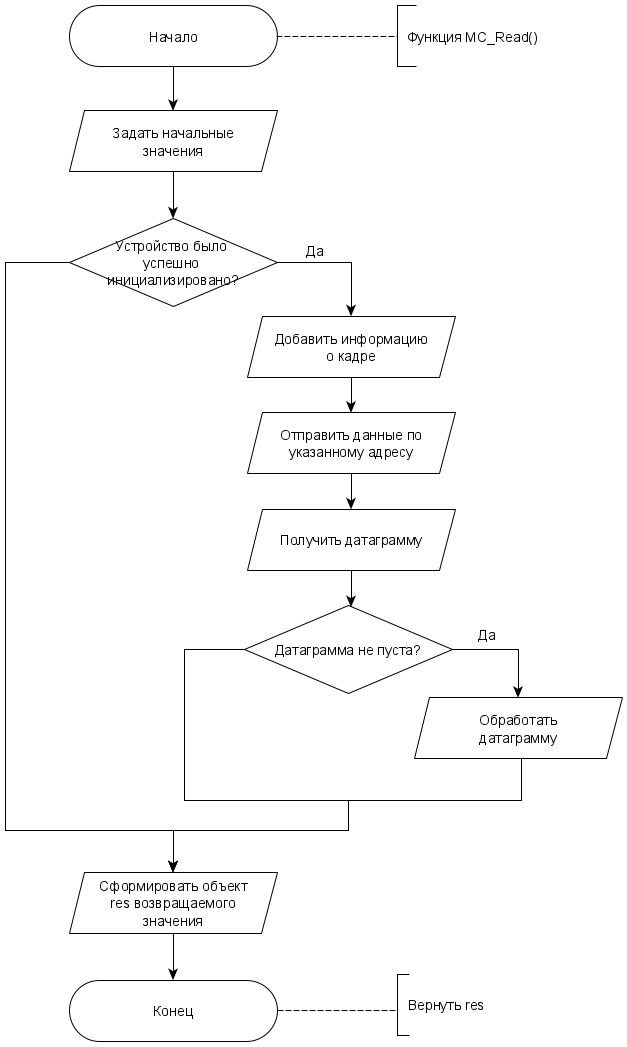
\includegraphics[scale=0.5]{schemes/mc_read.png}}
			\caption{MC$\_$Read()}
			\label{fig13:image}
		\end{center}
	\end{figure}

	\subsubsection{Функция инициализации сокета МКИО (Init)}
	
	Схема изображена на рисунке \ref{fig14:image}.
	
	\begin{figure}[ph!]
		\centering
		\begin{center}
			{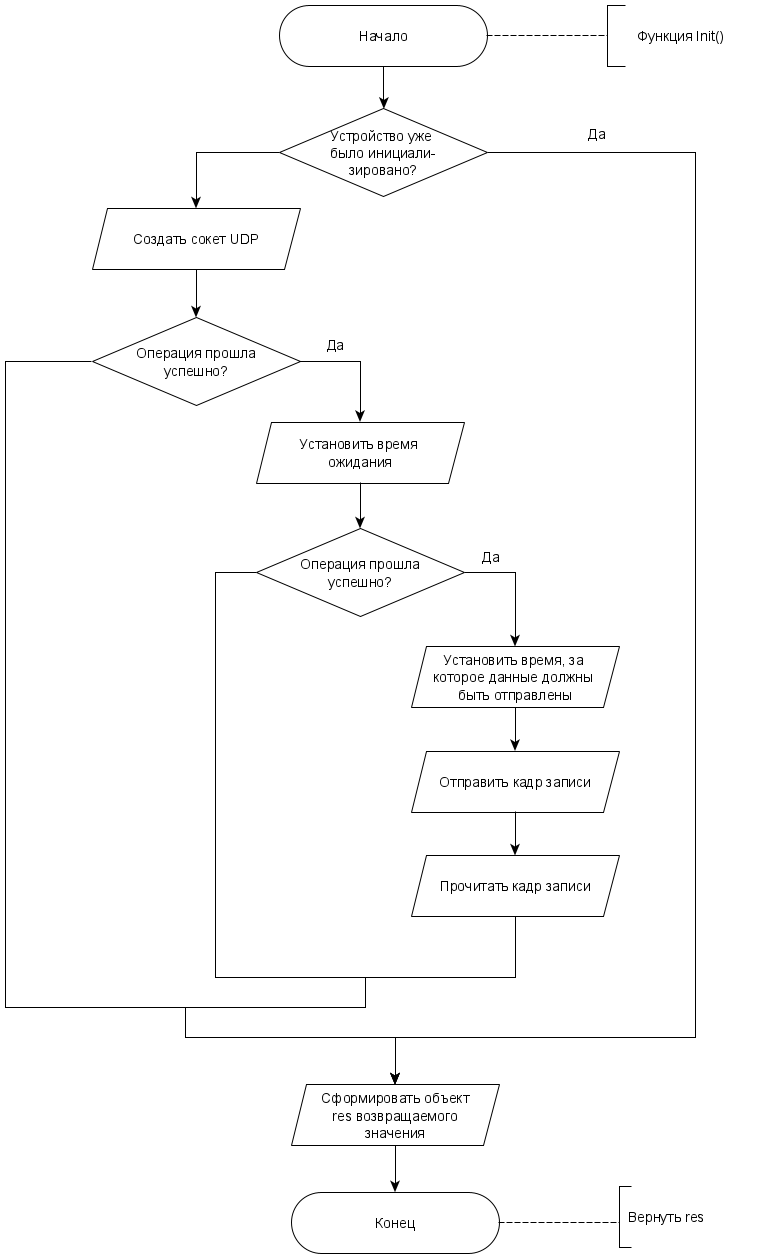
\includegraphics[scale=0.5]{schemes/init.png}}
			\caption{Init()}
			\label{fig14:image}
		\end{center}
	\end{figure}

	\subsubsection{Функция инициализации сокета КМБО (InitCom$\_$Kmbo)}
	
	Схема изображена на рисунке \ref{fig15:image}.
	
	\begin{figure}[ph!]
		\centering
		\begin{center}
			{\includegraphics[scale=0.5]{schemes/InitCom_Kmbо.png}}
			\caption{InitCom$\_$Kmbo()}
			\label{fig15:image}
		\end{center}
	\end{figure}

	\subsection{Вывод}
	В разделе приведены схемы основных функций, входящих в состав библиотеки.
